
%
\section{QuadTrack: a Dynamic 360{\textdegree} MOT Dataset}
\label{sec:QuadTrack}

%
Most existing MOT datasets~\cite{milan2016mot16,dendorfer2020mot20,peize2021dance} are captured using pinhole cameras, which are characterized by a narrow-FoV and linear sensor motion.
However, when panoramic-FoV capture devices experience even slight movements, the entire scene can change drastically, posing significant challenges for object tracking.
QuadTrack addresses this challenge by providing a benchmark specifically designed to test MOT algorithms under dynamic, non-linear motion conditions. 
%
It enables evaluating algorithm robustness in tracking objects with panoramic, non-uniform motion.
%

\subsection{Dataset Collection and Challenges}
To acquire a dataset with a panoramic FoV and complex motion dynamics, we utilized a quadruped robot dog as the data collection platform. This platform was selected for its biomimetic gait, which emulates the natural locomotion patterns of quadrupedal animals, introducing additional challenges for motion tracking due to its inherent complexity and variability. 
The robot measures $70cm{\times}31cm{\times}40cm$, with a maximum payload capacity of $7kg$. It can navigate vertical obstacles up to $15cm$ and inclines up to $30^{\circ}$, making it highly maneuverable in everyday environments. 
With $12$ joint motors, the robot replicates realistic walking motions at speeds up to $2.5m/s$.
For sensing, we used a Panoramic Annular Lens (PAL) camera to capture wide-angle scenes with a FoV of $360^\circ{\times}70^{\circ}$. 
The camera has a pixel size of $3.45{\mu}m{\times}3.45{\mu}m$, a resolution of $5$ million effective pixels, and supports a maximum output of $2048{\times}2048$ pixels at $40.5$FPS. 
Mounted on the quadruped robot (see Fig.~\ref{fig:robot_platform}~(b)), the camera ensures an unobstructed, optimal view. 
Using this platform, the outdoor data collection spans morning, noon, afternoon, and evening, in diverse unconstrained environments across five campuses in two cities.

With the biomimetic gait of the quadruped robot, the collected panoramic images naturally exhibited characteristic shaking, particularly along the Y-axis (Fig.~\ref{fig:robot_platform} (c) and (d)).
Compared to the JRDB dataset~\cite{martin2021jrdb}, our QuadTrack dataset introduces more complex motion challenges. Additionally, the data faces challenges such as uneven exposure, color inconsistencies due to the panoramic FoV, and increased motion blur, as rapid relative displacement between moving objects and the background intensifies the blurring effect. 
More details can be found in the supplementary.

\begin{figure}[!t]
  \centering
  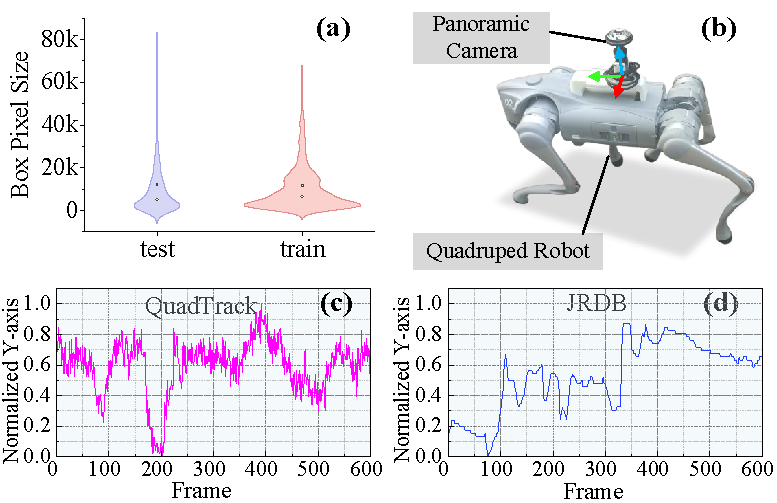
\includegraphics[width=0.48\textwidth]{imgs/robot_plat_v4.pdf}
  \vskip -2ex
  \caption{(a) shows the bounding box (bbox) size distribution for the training and validation sets, whereas (b) depicts the data collection platform and panoramic camera setup. (c) and (d) compare the normalized Y-axis pixel positions of trajectories between the QuadTrack~(\robotdog) and JRDB~\cite{martin2021jrdb}~(\robot) datasets, illustrating the significant vertical motion of the sensor in QuadTrack.}
  \label{fig:robot_platform}
  \vskip -2ex
\end{figure}
\subsection{Data Distribution and Comparative Analysis}
Unlike existing panoramic MOT datasets \cite{milan2016mot16,dendorfer2020mot20,geiger2013vision}, which rely on pinhole cameras, QuadTrack, as shown in Tab.~\ref{tab:comparison dataset}, is the first to be captured using a single $360^{\circ}$ panoramic camera. With a panoramic FoV ($360^{\circ}{\times}70^{\circ}$), QuadTrack significantly differs from traditional MOT datasets \cite{milan2016mot16,dendorfer2020mot20}. In contrast to autonomous driving datasets \cite{caesar2020nuscenes,bdd100k,waymo}, which often feature more predictable motion, QuadTrack incorporates complex, biologically inspired gait movements. Moreover, unlike internet-sourced datasets \cite{peize2021dance,cui2023sportsmot}, QuadTrack is designed to better reflect real-world application scenarios.
While many existing datasets~\cite{vipseg,waymo,caesar2020nuscenes,bdd100k} consist of short video sequences, QuadTrack emphasizes long-term tracking, with each video lasting $60$ seconds. To further challenge data association, we downsampled the dataset to $10$FPS, resulting in $600$ frames per sequence, spread across $32$ sequences. In total, QuadTrack includes $19,200$ frames and $189,876$ bounding boxes. 

%
As illustrated in Fig.~\ref{fig:robot_platform} (a), the distribution of both the training and test sets is consistent, ensuring a reliable and balanced evaluation of MOT methods. This similarity in the distribution between the sets reduces the potential for bias and allows for a more accurate comparison of model performance across varying conditions. The trajectories depicted in Fig.~\ref{fig:robot_platform} (c) and (d) highlight the increased complexity of multi-object tracking under panoramic FoV conditions. Notably, the motion along the Y-axis is significantly more intense compared to JRDB~\cite{martin2021jrdb}, further increasing the difficulty of object detection and association.
